\chapter{开波导点扩散函数分析}
\label{chap:req_b}
\section{定理\ref{thm_psf_half}的证明}
当反传播函数为$G_{k_1}(x,z):=\Phi_{k_1}(x,z)-\Phi_{k_1}(x,z')$时,点扩散函数$J(z,y)$为
\begin{equation}
  J(z,y)=\int_{\Gamma_0}\frac{\partial G_{k_1} (x,z)}{\partial x_2}\overline{N(x,y)}ds(x)
\end{equation}
其中$N(x,y)$为Pekeris开波导Neumann格林函数。根据引理\ref{lem:4.0}中关于Hankel函数$H_1^{(1)}(t)$的估计可知
\begin{equation}
 \left|\frac{\partial G_{k_1} (x,y)}{\partial x_2}\right|\leq C\frac{ k_1^{\frac{1}{2}}y_2}{|x-y|^{\frac{3}{2}}},\ \ x\in\Gamma_0,y\in\R^2_+
\end{equation}
从而点扩散函数$J(z,y)$是绝对收敛的。令$N_{\epsilon}(x,y)$是满足如下方程的波数为$k(x)+\i\epsilon$的格林函数:
\begin{eqnarray*}
\left\{
\begin{array}{lll}
  \Delta_x N_{\epsilon}(x,y)+[k(x)+\i\epsilon]^2N_{\epsilon}(x,y)=-\delta_y(x),&in&  \R_+^2\\
  & &\\
  \left[N_{\epsilon}(\cdot,y)\right]_{\Gamma_h}=\left[\frac{\partial N_{\epsilon}(\cdot,y)}{\partial x_2}\right]_{\Gamma_h}=0,\\
  & &\\
  \frac{\partial N_{\epsilon}(x,y)}{\partial x_2}=0,& on&\Gamma_0.
\end{array}
\right.
\end{eqnarray*}
令
\begin{equation}
    \hat{f}(\xi,x_2;y_1,y_2):=\int_{-\infty}^{\infty}f(x,y)e^{-\i x_1\xi}dx_1
\end{equation}
表示函数 $f(x,y)$ 关于$x$的的第一个分量的Fourier变换,则直接计算可得
\begin{eqnarray*}
\left\{
\begin{array}{lll}
   \frac{\partial \hat{G} (\xi,x_2;z_1,z_2)}{\partial x_2}\Big|_{x_2=0}&=&
   e^{\i\mu_1z_2-\i\xi z_1}\\
   & &\\
   \hat{N}_{\epsilon} (\xi,0;y_1,y_2)&=&\frac{\i}{\mu_{1\epsilon}}e^{\i\mu_{1\epsilon}y_2-\i\xi y_1}+
   \frac{\i}{\mu_{1\epsilon}}\frac{1}{\hat N_h^{\epsilon}(\xi)}\left[e^{\i\mu_{1\epsilon}(2h+y_2)-\i\xi y_1}+e^{\i\mu_{1\epsilon}(2h-y_2)-\i\xi y_1}\right]
\end{array}
\right.
\end{eqnarray*}
其中$\mu_{j\epsilon}=\sqrt{(k_j+\i\epsilon)^2-\xi^2},j=1,2$,以及
\begin{equation}
    \hat N_h^{\epsilon}(\xi)=
    \frac{\mu_{1\epsilon}+\mu_{2\epsilon}}{\mu_{1\epsilon}-\mu_{2\epsilon}}-e^{2\i\mu_{1\epsilon}h}
\end{equation}
直接验证可知,函数$\hat N_h^{\epsilon}(\xi)$在实轴上并不存在零点。令函数$J^{\epsilon}(z,y)$为
\begin{equation}
  J^{\epsilon}(z,y):=\int_{\Gamma_0}\frac{\partial G_{k_1}(x,z)}{\partial x_2}\overline {N^{\epsilon}(x,y)}ds(x),
\end{equation}
则根据Parseval恒等式,我们有
\begin{equation}
J^{\epsilon}(z,y)=\frac{1}{2\pi}\int_{-\infty}^{\infty}
   \left[\frac{\partial \hat{G} (\xi,x_2;z_1,z_2)}{\partial x_2}\cdot\overline{\hat{N}_{\epsilon} (\xi,x_2;y_1,y_2)}\right]_{x_2=0}d\xi
\end{equation}
于是函数$J^{\epsilon}(z,y)$的共轭$\overline{J^{\epsilon}(z,y)}$可以分为如下三个部分:
\begin{equation}
  \overline{J^{\epsilon}(z,y)}:=J^{\epsilon}_1(z,y)+J^{\epsilon}_2(z,y)+J^{\epsilon}_3(z,y)
\end{equation}
其中
\begin{eqnarray}
\left\{
\begin{array}{lll}
J^{\epsilon}_1(z,y)&=&\frac{\i}{2\pi}\int_{-\infty}^{+\infty}\frac{1}{\mu_{1\epsilon}}
e^{\i\mu_{1\epsilon}y_2-\i\overline\mu_1z_2+\i\xi(z_1-y_1)}d\xi\\
& &\\
J^{\epsilon}_2(z,y)&=&\frac{\i}{2\pi}\int_{-\infty}^{+\infty}\frac{1}{\mu_{1\epsilon}}
\frac{1}{\hat N_h^{\epsilon}(\xi)}
e^{\i\mu_{1\epsilon}(2h+y_2)-\i\overline\mu_1 z_2+\i\xi(z_1-y_1)}d\xi\\
& &\\
J^{\epsilon}_3(z,y)&=&\frac{\i}{2\pi}\int_{-\infty}^{+\infty}\frac{1}{\mu_{1\epsilon}}
\frac{1}{\hat N_h^{\epsilon}(\xi)}
e^{\i\mu_{1\epsilon}(2h-y_2)-\i\overline\mu_1 z_2+\i\xi(z_1-y_1)}d\xi
\end{array}
\right.
\end{eqnarray}
若令$J_1(z,y)=\lim\limits_{\epsilon\rightarrow0}J^{\epsilon}_1(z,y)$,则与文献\cite{ch_ha}中引理3.1一样,可得
\begin{equation}
  J_1(z,y)=F_1(z,y)+R_1(z,y)
\end{equation}
其中$|R_1(z,y)|< C(k_1h)^{-1}$,以及函数$F_1(z,y)$的共轭为
\begin{equation}
  \overline{F_1(z,y)}=-\frac{\i}{2\pi}\int_0^{\pi}e^{\i k_1(z_1-y_1)\cos\theta+\i k_1(z_2-y_2)\sin\theta}d\theta.
\end{equation}
下面我们只需说明下述估计即可:
\begin{equation}
 \left|\lim\limits_{\epsilon\rightarrow0}J^{\epsilon}_i(z,y)\right|<C\frac{k_1^2}{k_2^2}(k_1h)^{-\frac{1}{2}},\ \ i=2,3
\end{equation}
我们将以$J^{\epsilon}_2(z,y)$为例来说明上述估计。由定义可知:$J^{\epsilon}_2(z,y)=J^{\epsilon}_{2,1}(z,y)+J^{\epsilon}_{2,2}(z,y)$ ,其中
\begin{eqnarray*}
    J^{\epsilon}_{2,1}(z,y)&=&\frac{\i}{2\pi}\int_{-\infty}^{\infty}
        \frac{1}{\mu_{1\epsilon}}\frac{1}{\hat N_h^{\epsilon}(\xi)}e^{-\i \mu_1 z_2+\i\mu_{1\epsilon}(2h+y_2)+\i\xi(z_1-y_1)}d\xi\\
    J^{\epsilon}_{2,2}(z,y)&=&\frac{\i}{2\pi}\int_{\xi\in\R,|\xi|\geq k_1}
   \frac{1}{\mu_{1\epsilon}}\frac{1}{\hat N_h^{\epsilon}(\xi)}e^{\i\mu_{1\epsilon}(2h+y_2)+\i\xi(z_1-y_1)}
   \left[e^{\i\mu_1 z_2}-e^{-\i\mu_1 z_2}\right]d\xi
\end{eqnarray*}
我们首先来估计第二项,注意到当$\epsilon\rightarrow0$时,极限$\lim\limits_{\epsilon\rightarrow0}J^{\epsilon}_{2,2}(z,y)$是存在且收敛的,记为$J_{2,2}(z,y)$,则
\begin{equation}
  J_{2,2}(z,y)=\frac{\i}{2\pi}\int_{\xi\in\R,|\xi|\geq k_1}
   \frac{1}{\mu_1}\frac{1}{\hat N_h(\xi)}e^{\i\mu_1(2h+y_2)+\i\xi(z_1-y_1)}
   \left[e^{\i\mu_1 z_2}-e^{-\i\mu_1 z_2}\right]d\xi
\end{equation}
注意到当$\xi\in\R,|\xi|\geq k_1$时,$|\hat N_h(\xi)|\geq 1$,然后直接估计可得:
\begin{equation}
  | J_{2,2}(z,y)|\leq C(k_1h)^{-1}
\end{equation}
其中常数$C>0$与$k_1,k_2,h$无关。现在我们来看第一项:$J^{\epsilon}_{2,1}(z,y)$。由于当$\epsilon=0$时,函数$\hat N_h(\xi)$ 在实轴上存在一阶零点,故而类似于正文推导的各种格林函数,我们在令$\epsilon\rightarrow0$之前,需要利用Cauchy积分定理将其化到如图\ref{SIP_path4}所示的SIP 积分路径上,然后记$\epsilon\rightarrow0$ 的极限为$J_{2,1}(z,y)$,则
\begin{equation}
  J_{2,1}(z,y)=\frac{\i}{2\pi}\int_{SIP}
        \frac{1}{\mu_1}\frac{1}{\hat N_h(\xi)}e^{\i\mu_1(2h+y_2-z_2)+\i\xi(z_1-y_1)}d\xi
\end{equation}
\begin{figure}
  \centering
  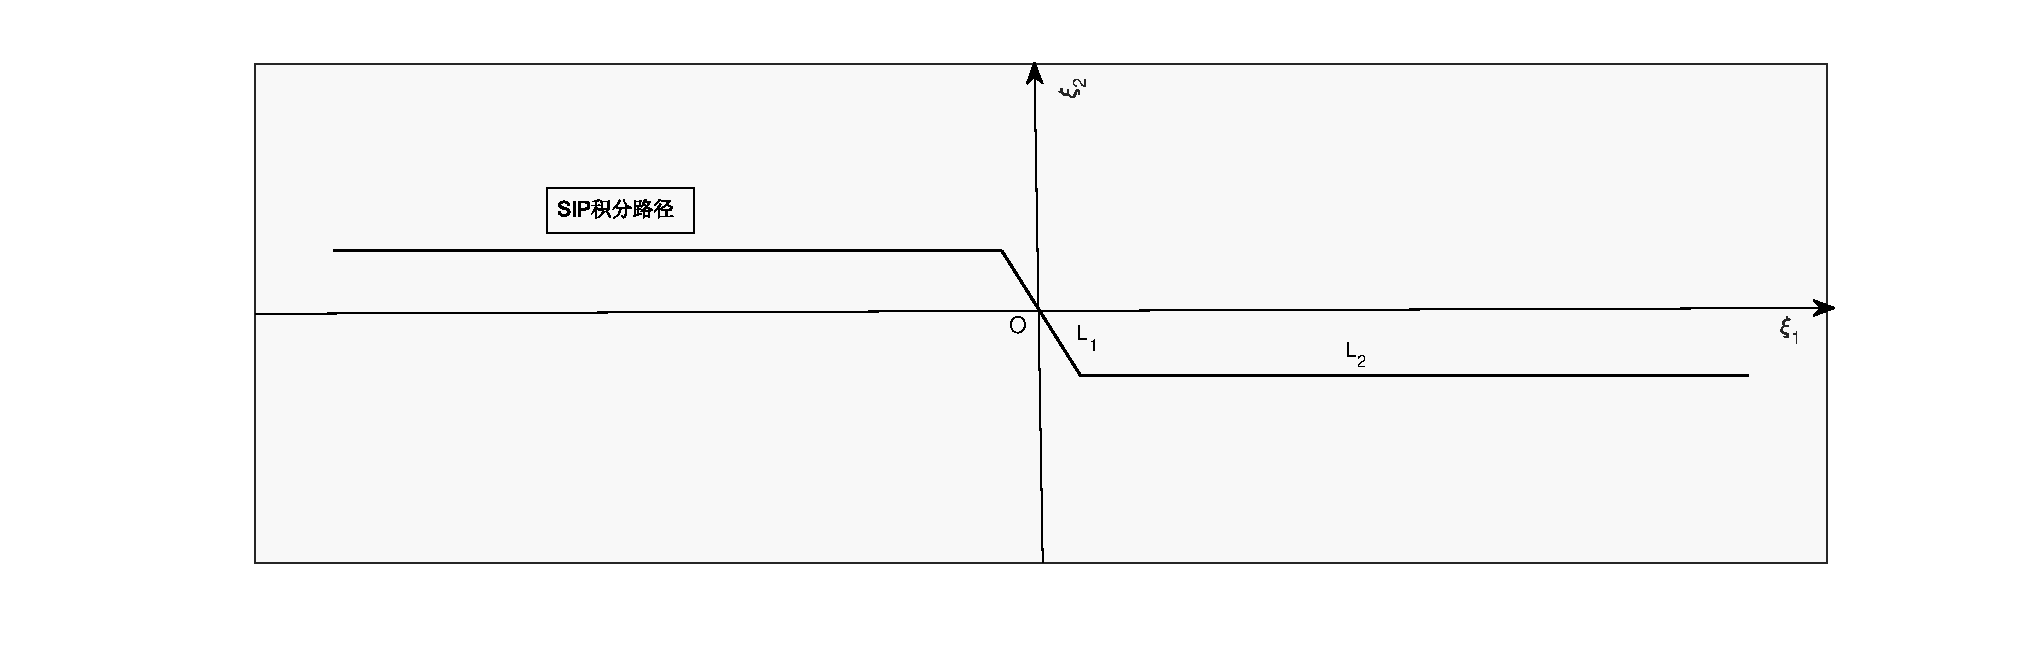
\includegraphics[width=15cm,height=6cm]{./SIP/SIP_path.eps}
  \caption{SIP积分路径}\label{SIP_path4}
\end{figure}

类似于文献\cite{ch_cw}中的定理4.2,关于上述类型的SIP积分,我们可以证明下述引理。
\begin{lemma}\label{SIP_estimate}
假设存在$\alpha_1,\alpha_2\in(0,1)$ 使得
\begin{equation}
  0<a\leq\alpha_1h,\ \ 0<k_1b\leq\alpha_2\sqrt{k_1h},
\end{equation}
 则存在与$k_1,k_2,h$无关的常数$C>0$使得
\begin{equation}
    |\Theta(a,b)|\leq C\frac{k_1^2}{k_2^2}\frac{1}{\sqrt{k_1h}}.
\end{equation}
其中
\begin{eqnarray}
 \Theta(a,b)=\int_{SIP}\frac{1}{\mu_1}\frac{1}{\hat N_h(\xi)}e^{\i\mu_1a+\i\xi b}d\xi
\end{eqnarray}
\end{lemma}
\debproof
令 $\gamma=\frac{1}{\sqrt{2k_1h}}$,以及$SIP^+=L_1\cup L_2$,其中
$$
 L_1=\{\xi\in\mathbb{C}: \xi_1\in(0,k_1\gamma), \xi_2=-\xi_1\},\ \
 L_2=\{\xi\in\mathbb{C}: \xi_1\in(k_1\gamma,+\infty), \xi_2=-k_1\gamma\}
.$$
通过在第二象限做如下变换:$\xi\rightarrow-\xi$, 我们便可以将$\Theta(a,b)$化为$SIP^+$上的如下积分:
\begin{equation}
\Theta(a,b)=\int_{SIP^+} \frac{1}{\mu_1}\frac{1}{\hat N_h(\xi)}
e^{\i\mu_1a}\left[e^{\i\xi b}+e^{-\i\xi b}\right]d\xi\quad
\end{equation}
记$\mu_1:=\mu_{1r}+\i\mu_{1i}$,则在第四象限
$$
|\mu_1|^2=\sqrt{(k_1^2-\xi_1^2+\xi_2^2)^2+4\xi_1^2\xi_2^2},\ \ \mu_{1r}=\sqrt{\frac{|\mu_1|^2+(k_1^2-\xi_1^2+\xi_2^2)}{2}},\ \ \mu_{1i}=\frac{\sqrt{2}\xi_1|\xi_2|}{\sqrt{|\mu_1|^2+(k_1^2-\xi_1^2+\xi_2^2)}} $$
关于$\mu_2=\sqrt{k_2^2-\xi^2}$ 有类似的表达式。 更进一步, 在 $L_1$上
$$
|\mu_1|^2=\sqrt{k_1^4+4\xi_1^4},\ \
\mu_{1r}=\sqrt{\frac{|\mu_1|^2+k_1^2}{2}},\ \
\mu_{1i}=\frac{\sqrt{2}\xi_1^2}{\sqrt{|\mu_1|^2+k_1^2}}
$$
再注意到在$L_1$上,$\mu_{1r}\geq\mu_{2r}$ 及 $\mu_{1i}\leq\mu_{2i}$,我们便可以得到
\begin{eqnarray*}
|\mu_1+\mu_2|^2-|\mu_1-\mu_2|^2=4(\mu_{1r}\mu_{2r}+\mu_{1i}\mu_{2i})\geq4(\mu_{2r}^2+\mu_{1i}^2)
\end{eqnarray*}
于是在 $L_1$上
\begin{eqnarray*}
 \left|\frac{1}{\hat N_h(\xi)}\right|&=&\left|\frac{\mu_1-\mu_2}{\mu_1+\mu_2+(\mu_2-\mu_1)e^{2\i\mu_1h}}\right|\\
&\leq&\frac{|\mu_1-\mu_2|}{|\mu_1+\mu_2|-|\mu_1-\mu_2|}\\
&=&\frac{|\mu_1-\mu_2|(|\mu_1+\mu_2|+|\mu_1-\mu_2|)}{4(\mu_{1r}\mu_{2r}+\mu_{1i}\mu_{2i})}\\
&\leq&\frac{2\mu_1^2}{\mu_{2r}^2+\mu_{1i}^2}\leq \frac{2\sqrt2 k_1^2}{k_2^2}
\end{eqnarray*}
上述不等式最后一步我们用到如下估计:
\begin{eqnarray*}
\mu_{2r}^2+\mu_{1i}^2=\frac{1}{2}\{|\mu_2|^2+k_2^2+|\mu_1|^2-k_1^2\}\geq k_2^2,\ \ on \ \ L_1.
\end{eqnarray*}
下面我们来看在$L_2$的估计,注意到在$L_2$上,直接计算可得
$|\mu_1|^2\leq k_1^2+\xi_1^2+\xi_2^2$,以及
\begin{eqnarray*}
\mu_{1i}h\geq\frac{\xi_1|\xi_2|h}{\sqrt{k_1^2+\xi_2^2}}=\frac{\xi_1h\gamma}{\sqrt{1+\gamma^2}}\geq\frac{k_1h\gamma^2}{\sqrt2}=\frac{1}{2\sqrt2}
,\ \ on \  \ L_2.
\end{eqnarray*}
从而
\begin{eqnarray*}
\left|\frac{1}{\hat N_h(\xi)}\right|=
\frac{1}{\left|\frac{\mu_1+\mu_2}{\mu_1-\mu_2}-e^{2\i\mu_1h}\right|}\leq
\frac{1}{1-e^{-2\mu_{1i}h}}\leq\frac{1}{1-e^{-1/\sqrt2}}
\end{eqnarray*}
根据关于$a,b$的假设可得:
$$
\left|e^{\i\xi b}+e^{-\i\xi b}\right|\leq2e^{-\xi_2 b}\leq 2e^{\alpha_2/\sqrt2},\ \ \forall\xi\in L_1\cup L_2.
$$
以及
$$\left|e^{\i\mu_1 a}\right|\leq e^{-\alpha_1\mu_{1i}h},\ \ \forall\xi\in L_1\cup L_2.$$
从而
\begin{equation}
\left|\Theta(a,b)\right|\leq C\left|\int_{L_1\cup L_2}\frac{1}{|\mu_1|}\left|\frac{1}{\hat N_h(\xi)}\right|e^{-\alpha_1\mu_{1i}h}d\xi\right|.
\end{equation}
注意到在$L_1$上,$|\mu_1|\geq k_1$,然后直接估计即可得
\begin{eqnarray*}
\left|\int_{L_1}\frac{1}{|\mu_1|}\left|\frac{1}{\hat N_h(\xi)}\right|e^{-\alpha_1\mu_{1i}h}d\xi\right|
\leq C\frac{k_1^2}{k_2^2}\gamma\leq C\frac{k_1^2}{k_2^2}\frac{1}{\sqrt{k_1h}},
\end{eqnarray*}
至于在$L_2$上的估计,结合关于函数$\hat N_h(\xi)$的估计,直接放缩可得
\begin{eqnarray*}
\left|\int_{L_2}\frac{1}{|\mu_1|}\left|\frac{1}{\hat N_h(\xi)}\right|e^{-\alpha_1\mu_{1i}h}d\xi\right|
\leq C\int_{k_1\gamma}^{+\infty}\frac{1}{|\mu_1|}e^{-\alpha_1\mu_{1i}h}d\xi_1.
\end{eqnarray*}
关于上式右端的估计,文献\cite{ch_cw}中定理4.2有类似的分析。为保证证明完整性,我们简要说明一下估计过程。首先注意到
\begin{equation*}
 \mu_{1i}\geq\frac{\xi_1|\xi_2|}{\sqrt{k_1^2+\xi_2^2}}=\frac{\xi_1\gamma}{\sqrt{1+\gamma^2}}\geq\frac{\xi_1\gamma}{\sqrt2}
,\ \ on \  \ L_2.
\end{equation*}
然后将区间$(k_1\gamma,+\infty)$分为两段:$(k_1\gamma,k_1/\sqrt{2\pi})$和$(k_1/\sqrt{2\pi},+\infty)$,然后
\begin{itemize}
  \item 当$\xi_1\in(k_1\gamma,k_1/\sqrt{2\pi})$时,$|\mu_1|\geq\sqrt{k_1^2-\xi_1^2}\geq k_1\sqrt{1-\frac{1}{2\pi}}$,
  \item 当$\xi_1\in(\frac{k_1}{\sqrt{2\pi}},+\infty)$时,$|\mu_1|\geq\sqrt{2{\xi_1|\xi_1|}}\geq\sqrt[4]{\frac{2}{\pi}}k_1\gamma$,
\end{itemize}
于是
\begin{eqnarray*}
\int_{k_1\gamma}^{+\infty}\frac{1}{|\mu_1|}e^{-\alpha_1\mu_{1i}h}d\xi_1&=&
\int_{k_1\gamma}^{\frac{k_1}{\sqrt{2\pi}}}\frac{1}{|\mu_1|}e^{-\alpha\mu_{1i}h}d\xi_1
+\int_{\frac{k_1}{\sqrt{2\pi}}}^{+\infty}\frac{1}{\mu_1}e^{-\alpha_1\mu_{1i}h}d\xi_1\\
&\leq&\frac{C}{k_1}\int_{k_1\gamma}^{\frac{k_1}{\sqrt{2\pi}}}e^{-\frac{\alpha_1}{2}\frac{\xi_1h}{\sqrt{k_1h}}}d\xi_1
+\frac{C}{k_1\gamma^{1/2}}\int_{\frac{k_1}{\sqrt{2\pi}}}^{+\infty}e^{-\frac{\alpha_1}{2}\frac{\xi_1h}{\sqrt{k_1h}}}d\xi_1\\
&=&-\frac{C}{k_1h}\left[e^{-\frac{\alpha_1}{2}\frac{\xi_1h}{\sqrt{k_1h}}}\right]\Bigg|_{k_1\gamma}^{\frac{k_1}{\sqrt{2\pi}}}
-\frac{C}{\sqrt[4]{k_1h}}\left[e^{-\frac{\alpha_1}{2}\frac{\xi_1h}{\sqrt{k_1h}}}\right]\Bigg|_{\frac{k_1}{\sqrt{2\pi}}}^{+\infty}\\
&\leq&C\frac{1}{{\sqrt{k_1h}}}.
\end{eqnarray*}

综合上述估计,最终我们得到:$\left|\Theta(a,b)\right|\leq C\frac{k_1^2}{k_2^2}(k_1h)^{-1/2}$.
\finproof

由引理\ref{SIP_estimate}可知,$\left|J_{2,1}(z,y)\right|<C\frac{k_1^2}{k_2^2}(k_1h)^{-\frac{1}{2}}$,然后类似地,我们可以处理$J_3^{\epsilon}(z,y)$。最后结合$J_1(z,y)$的估计,我们便完成了定理\ref{thm_psf_half}的证明。
